% Version 3.1 December 2024
\documentclass[pdflatex,sn-mathphys-num]{sn-jnl}

\usepackage{graphicx}
\usepackage{multirow}
\usepackage{amsmath,amssymb,amsfonts}
\usepackage{amsthm}
\usepackage{mathrsfs}
\usepackage[title]{appendix}
\usepackage{xcolor}
\usepackage{textcomp}
\usepackage{manyfoot}
\usepackage{booktabs}
\usepackage{algorithm}
\usepackage{algorithmicx}
\usepackage{algpseudocode}
\usepackage{listings}
\usepackage{url}

\lstset{
  breaklines=true,
  basicstyle=\ttfamily\small,
  columns=fullflexible
}

\raggedbottom

\theoremstyle{thmstyleone}
\newtheorem{theorem}{Theorem}
\newtheorem{proposition}[theorem]{Proposition}
\theoremstyle{thmstyletwo}
\newtheorem{example}{Example}
\newtheorem{remark}{Remark}
\theoremstyle{thmstylethree}
\newtheorem{definition}{Definition}

\begin{document}

\title[Heterogeneous Agentic AI System Using Fine-Tuned SLMs]{Heterogeneous Agentic AI System Using Fine-Tuned SLMs}

\author*[1]{\fnm{Arsh} \sur{}}\email{arsh03.2005@gmail.com}
\author[2]{\fnm{Swarnendu} \sur{Ghosh}}
\author[1]{\fnm{Akshay} \sur{Rajput}}

\affil*[1]{\orgdiv{Department of Computer Science and Engineering}, \orgname{Graphic Era (Deemed to be University)}, \orgaddress{\city{Dehradun}, \country{India}}}

\affil[2]{\orgdiv{AI Research Division}, \orgname{StartHack.IO Pvt Ltd}, \orgaddress{\city{Dehradun}, \country{India}}}

\abstract{This paper introduces a heterogeneous agentic AI architecture that leverages fine-tuned Small Language Models (SLMs) for efficient, context-aware UI component generation. Unlike general-purpose LLM approaches that entail heavy computational loads and lack task specificity, the proposed model employs Gemma~4~E2B, a lightweight general-purpose SLM with 2.3B effective parameters, to tokenize user requests and transfer section-level generation tasks to Qwendean, our SLM fine-tuned from Qwen3-4B and specialized in the UI domain. A set of more than 900 UI components collected from ShadCN and TailwindCSS was augmented with synthetic prompt–completion pairs generated using DeepSeek models. After three augmentation passes the data increased to over 4100 samples and was released as \texttt{iamdyeus/ui-instruct-4k} on Hugging Face. Fine-tuning was performed using rsLoRA at 16-bit precision. The final pipeline, orchestrated by LangGraph, produces complete functioning React/TypeScript pages. Empirical results show that the heterogeneous design yields better cohesion, lower inference latency (3–5\,s per section), near-zero API costs, and higher stylistic consistency compared to homogeneous LLM baselines. We further demonstrate that functional specialization—rather than model scale—is the key to efficient agentic AI.}

\keywords{Agentic AI, Small Language Models, Fine-Tuning, rsLoRA, UI Code Generation, LangGraph, ShadCN, TailwindCSS, Heterogeneous AI Systems}

\maketitle

\section{Introduction}\label{sec:intro}

The agentic AI paradigm represents a new trend in artificial intelligence in which agents break down complex tasks into smaller ones and carry them out efficiently~\cite{ref1}. Unlike traditional generative AI that produces single-step outputs, agentic models incorporate planning and tool use for multi‑step reasoning and execution~\cite{ref2}. While larger orchestrator models show higher competence in reasoning and task decomposition, they suffer from lower speeds and cost inefficiency. Narrow tasks such as creating an icon or a hero section do not require such heavy capabilities.

Small Language Models (SLMs) have recently become popular as alternatives to LLMs for specific operations within an agentic architecture. As noted in recent research~\cite{ref1}, SLMs offer substantial advantages in heterogeneous systems: lower computation cost, faster inference, and the possibility of fine‑tuning for precise applications. These benefits become crucial when latency, cost, and scalability are considered. Importantly, the advantage does not depend solely on model size but on functionality.

This paper argues—and demonstrates empirically—that a heterogeneous agentic architecture, where a general‑purpose SLM handles orchestration and a domain‑specialized fine‑tuned SLM handles generation, outperforms homogeneous architectures where a single model performs both roles. Our architecture employs Gemma~4~E2B as a lightweight requirements gatherer and task planner, paired with Qwendean (fine‑tuned Qwen3-4B) as a specialized UI code generator. The advantages go beyond cost: the specialized model produces outputs better aligned with the target domain in syntactic validity and stylistic coherence, while the general‑purpose model is more effective at query decomposition without resorting to supercomputers.

We implement this framework for automated web UI component generation. Our key contributions are:
\begin{enumerate}
    \item A systematic three‑round iterative pipeline for collecting, normalising, annotating and augmenting UI component datasets, increasing from 900 to over 4100 high‑quality training examples from open‑source libraries.
    \item A synthetic prompt generation methodology using DeepSeek-V3 to produce diverse, context‑aware prompt–completion pairs in JSONL format, published as \texttt{iamdyeus/ui-instruct-4k} on Hugging Face.
    \item Qwendean: a LoRA fine‑tuned version of Qwen3-4B using rank‑stabilized LoRA (rsLoRA) with 16‑bit precision, proving that a 4B model fine‑tuned on specific data can generate production‑ready React/TypeScript/ShadCN/Tailwind components with significantly higher consistency than general‑purpose models.
    \item Demonstration that lightweight general‑purpose models suffice for orchestration in scope‑controlled agentic systems; diversity of specialisations, not model size, is responsible for efficiency.
    \item A heterogeneous agentic pipeline orchestrated by LangGraph, where Gemma~4~E2B decomposes a user page request into section‑level prompts, sends them to Qwendean for generation, and assembles the final page.
    \item An iterative analysis of overfitting, dataset quality and training dynamics across three training rounds, offering practical insights for future SLM fine‑tuning in code generation.
\end{enumerate}

\begin{figure}[htbp]
\centering
\includegraphics[width=\linewidth]{images/image1.png}
\caption{Overall heterogeneous agentic architecture}
\label{fig:architecture}
\end{figure}

\section{Related Work}\label{sec:related}

\subsection{Agentic AI and Task Orchestration}
Agentic AI extends generative models with autonomy and tool use. Frameworks such as LangGraph and AutoGen enable multi‑agent architectures where specialised agents collaborate on complex tasks~\cite{ref3}. Key features include task decomposition, memory/planning, and tool invocation. Recent studies highlight resource conservation when small models handle recurring tasks~\cite{ref1}.

\subsection{Small Language Models in Specialised Domains}
Smaller models (under 10 B parameters) can perform well on code generation and mathematical reasoning when properly fine‑tuned~\cite{ref4}. Qwen models show strong results in code understanding and generation; Qwen3-4B offers a favourable balance between capacity and computational requirements~\cite{ref5}. Small general‑purpose models can perform complex reasoning if properly scaffolded. Specialisation‑based heterogeneity (generalist vs. domain expert) yields better efficiency than scale‑based heterogeneity (large vs. small) for functionally decomposable tasks.

\subsection{LoRA and Quantised Fine‑Tuning}
Low‑Rank Adaptation (LoRA)~\cite{ref12} injects trainable low‑rank matrices into transformer layers, reducing trainable parameters. QLoRA~\cite{ref13} quantises the base model to 4‑bit NF4, further reducing memory. Rank‑Stabilised LoRA (rsLoRA)~\cite{ref17} normalises the scaling factor by $\sqrt{r}$ instead of $r$, stabilising training at higher ranks ($r=32$ and above). We employ rsLoRA throughout because structured code generation benefits from increased rank capacity.

\subsection{Synthetic Data Generation for Fine‑Tuning}
Recent approaches use synthetic prompt generation to create diverse, realistic prompts~\cite{ref6}, preference optimisation (DPO)~\cite{ref7} to align outputs without reward models, and multi‑stage pipelines with reasoning and critique models~\cite{ref8}. Our approach follows this paradigm, using DeepSeek-V3 for component description and synthetic prompt construction.

\subsection{UI Component Libraries and Code Generation}
Modular UI frameworks (ShadCN, TailwindCSS, Radix UI) provide reusable building blocks. Automating their selection and adaptation to specific contexts is an open challenge~\cite{ref9}. Existing systems either rely on monolithic LLMs (costly and slow) or brittle rule‑based heuristics. Our heterogeneous approach bridges this gap by combining planning with specialised fine‑tuned generation.

\subsection{Gaps in Current Literature}
Few works combine LLMs and agentic systems in an end‑to‑end, empirically rigorous manner. Specifically, the literature lacks:
\begin{enumerate}
    \item Analysis of data size and source heterogeneity effects on LLM‑generated code quality through iterative training.
    \item Investigation of overfitting during fine‑tuning on small code datasets.
    \item Integration of fine‑tuned LLMs as specialised agents in graph‑based orchestration platforms.
\end{enumerate}
This paper addresses all three gaps.

\section{Problem Statement}\label{sec:problem}

Traditional automatic code/content creation suffers from fundamental shortcomings that hinder production‑level use, regardless of whether large LLMs or general‑purpose SLMs are employed.

\paragraph{Absence of Domain Specialisation}
General‑purpose models (70B LLMs or 7B SLMs) cannot specialise output to domain‑specific constraints. When asked to create a React component, there is no guarantee that ShadCN primitives, Tailwind classes, or project‑specific guidelines will be used. Even general‑purpose SLMs lack an adequate understanding of idiomatic syntax unless explicitly prompted.

\paragraph{Computational Inefficiency of Monolithic Architecture}
Systems where a single model handles both orchestration and execution cannot optimise separately for these two activities. Orchestration (logical reasoning in a limited domain) suits lightweight general‑purpose models, while coding requires deep specialisation (internal patterns, naming conventions, library‑specific APIs). Coupling both forces them into the computational constraints of the latter.

\paragraph{Wasted Computational Resources in Latent Operations}
Using one large model for all tasks wastes compute resources. Even using one general‑purpose model for both roles yields poorer results than using a separate generalist planner and fine‑tuned domain specialist—not only due to computation but because of output quality differences.

\paragraph{Context Loss and Inconsistency}
General‑purpose models produce outputs that depend on exact prompt wording; different phrasings lead to different styles, structures, and inconsistencies. A fine‑tuned domain specialist produces consistent style, predictable structure, and conformance to library idioms.

\section{Methodology}\label{sec:methodology}

\subsection{Dataset Construction: Iterative Development}

The dataset evolved across three rounds (Fig.~\ref{fig:dataset}), each motivated by observed training behaviour.

\subsubsection{Initial Collection (900+ components)}
We collected UI components from ShadCN UI and TailwindCSS using automated scraping, extracting over 900 distinct components (hero sections, feature lists, navbars, footers, testimonials, cards, modals). A standardisation process (code formatting, dependency management, metadata extraction, quality assessment) produced more than 900 validated components. Initial fine‑tuning on this corpus led to severe overfitting—the model memorised training samples but produced redundant or gibberish responses.

\subsubsection{Prompt Augmentation (2,400+ samples)}
To address overfitting, we generated multiple prompt variants per existing component using DeepSeek-V3~\cite{ref6}. Each component's code and metadata produced a baseline natural‑language query, which was elaborated via chain‑of‑thought reasoning incorporating industry context, visual vibe, and accessibility. This yielded about 2,400 training rows. Overfitting decreased, and the model began generating more diverse outputs, but quality remained suboptimal (incorrect API merges, outdated Tailwind syntax, poor prompt alignment).

\subsubsection{Multi‑Library Expansion (4,100+ samples)}
We expanded the source corpus with publicly available UI libraries (Aceternity UI, Magic UI, etc.) that follow the ShadCN design language, sourced from GitHub based on stars and activity. This added new archetypes, improved React/TypeScript idioms, and increased style diversity without diverging from ShadCN. The expanded corpus went through the same two‑stage synthetic prompt pipeline, producing a final dataset of approximately 4,100 samples (90/10 train/validation split), released as \texttt{iamdyeus/ui-instruct-4k}. Training on this dataset substantially improved output coherence, idiomatic correctness, and semantic alignment.

\begin{figure}[htbp]
\centering
\includegraphics[width=\linewidth]{images/image2.png}
\caption{Dataset evolution pipeline across three rounds}
\label{fig:dataset}
\end{figure}

\subsection{JSONL Dataset Format}
All training data is stored in JSONL format (standard for Hugging Face, Unsloth):
\begin{lstlisting}
{"prompt": "<DESCRIBE THE COMPONENT>", "completion": "<GENERATED CODE OR OUTPUT>"}
\end{lstlisting}

\subsection{Model Selection and Fine‑Tuning Configuration}
We selected Qwen3-4B as the base SLM for:
\begin{itemize}
    \item Competitive code generation performance.
    \item 4B parameter scale (efficient on consumer GPUs, 8–10 GB VRAM for FP16 inference).
    \item Open‑source (Apache 2.0) via Hugging Face.
    \item Dual reasoning modes (thinking mode disabled to produce clean code‑only output).
\end{itemize}

The model was loaded in 16‑bit (bfloat16) precision without quantisation, using Unsloth's FastLanguageModel with gradient checkpointing. Although QLoRA~\cite{ref13} was evaluated, it introduced syntax‑level artifacts in code generation and was not adopted.

LoRA adapters were configured with rsLoRA:
\begin{itemize}
    \item Rank $r=32$, alpha $=32$, dropout $=0.0$.
    \item Target modules: \texttt{q\_proj, k\_proj, v\_proj, o\_proj} (attention) and \texttt{gate\_proj, up\_proj, down\_proj} (MLP).
    \item rsLoRA enabled: scaling factor normalised by $\sqrt{r}$ for stability.
\end{itemize}

Training hyperparameters:
\begin{itemize}
    \item Batch size: per device 2, gradient accumulation 8, effective batch size 16.
    \item Epochs: 3.
    \item Learning rate: $1\times10^{-4}$, linear decay, warmup 16 steps.
    \item Optimizer: AdamW 8‑bit, weight decay 0.01.
    \item Max sequence length: 4096 tokens.
    \item Evaluation every 50 steps, early stopping patience 3, best checkpoint loaded.
    \item Packing disabled to avoid mid‑code truncation artifacts.
\end{itemize}

Training used an NVIDIA RTX 6000 PRO. After training, LoRA adapters were merged into the base model and pushed to Hugging Face in merged\_16bit precision, with additional GGUF quantisations for Ollama/LM Studio.

\begin{figure}[htbp]
\centering
\includegraphics[width=\linewidth]{images/image3.png}
\caption{Training pipeline}
\label{fig:training-pipeline}
\end{figure}

\subsection{Agent Architecture System}
We designed a heterogeneous agentic system for UI page generation with three logical layers: Orchestration, Execution, and Assembly/Validation, implemented using LangGraph for graph‑based workflow management.

\subsubsection{Orchestration Layer}
Gemma~4~E2B (2B parameters) acts as the requirements gatherer and orchestrator. Given a high‑level user command (e.g., “Create a SaaS landing page for a fintech product for enterprise customers”), the orchestrator engages in a conversational dialogue to resolve ambiguities (visual style, target audience, sections, colour scheme, accessibility). After clarification, it performs task decomposition using chain‑of‑thought prompting, producing an ordered list of section IDs with metadata‑enriched prompts (industry, vibe, colour theme, accessibility). The orchestrator’s lightweight nature validates that logical reasoning in a bounded domain does not require a large model.

\subsubsection{Execution Layer}
Each section prompt is routed to Qwendean, the fine‑tuned Qwen3-4B domain specialist. Qwendean receives the prompt along with a system prompt instructing clean React/TypeScript code using ShadCN and Tailwind, with thinking mode disabled (code‑only output). LangGraph routes via conditional edges: the orchestrator node updates the shared state with the section list and maps each section to the Qwendean node sequentially.

\subsubsection{Assembly and Validation Layer}
A synthesizer node concatenates the generated sections, resolves import deduplication, ensures consistent prop types across shared components, and applies a final layout wrapper. A rubric‑based validation step checks syntactic validity, correct ShadCN API usage, Tailwind class correctness, and vibe consistency. Sections that fail are flagged for regeneration (max three attempts) or send back to the orchestrator for prompt refinement.

\begin{figure}[htbp]
\centering
\includegraphics[width=\linewidth]{images/image4.png}
\caption{Detailed agentic architecture flow (LangGraph implementation)}
\label{fig:agentic-flow}
\end{figure}

\section{Results and Discussion}\label{sec:results}

\subsection{Training Dynamics Across Iterations}
Three rounds clearly showed that dataset diversity is more important than raw size.
\begin{itemize}
    \item \textbf{Round 1 (900 samples):} Training loss dropped to near zero, validation loss rose after ~60 steps → severe overfitting. Outputs were often gibberish.
    \item \textbf{Round 2 (2,400 samples):} Train‑validation gap narrowed; overfitting postponed. However, systematic mistakes remained: incorrect ShadCN props, confusion between Tailwind v3 and v4 classes, valid structure but wrong content.
    \item \textbf{Round 3 (4,100 samples):} Validation loss declined smoothly over 3 epochs; early stopping fired later, indicating continued meaningful learning. Qualitative evaluation showed correct ShadCN API usage, idiomatic Tailwind classes, and clean assembly without manual fixes.
\end{itemize}

\begin{figure}[htbp]
\centering
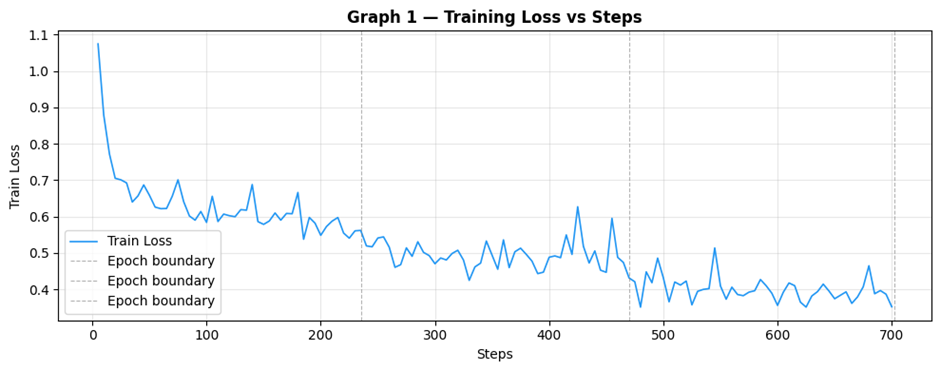
\includegraphics[width=0.8\linewidth]{images/training_loss.png} % assume you have these images
\caption{Training loss decreasing over steps (Round~3)}
\label{fig:loss}
\end{figure}

\begin{figure}[htbp]
\centering
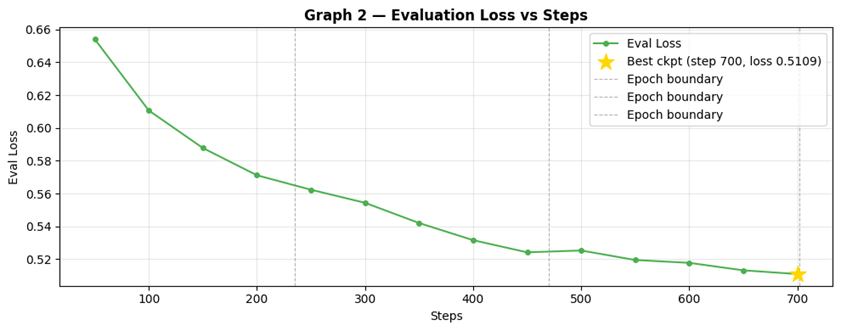
\includegraphics[width=0.8\linewidth]{images/eval_loss.png}
\caption{Training and validation loss comparison}
\label{fig:eval-loss}
\end{figure}

\subsection{Model Configuration Insights}
rsLoRA at rank 32 was crucial. Preliminary experiments with standard LoRA (rank 16) showed unstable gradient norms during the first epoch. Switching to rsLoRA produced stable gradient norms, a smooth learning rate decay, and a minimum validation loss of 0.5109 at step 700.

Training in 16‑bit precision (instead of 4‑bit QLoRA) improved output quality at the cost of higher VRAM (24–32 GB total). The 4‑bit approach introduced quantisation noise that caused syntactic issues in long completions. Sequence length 4096 covered the 99th percentile of training samples; packing was disabled to avoid truncated partial completions.

\begin{figure}[htbp]
\centering
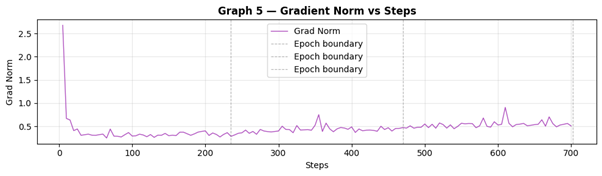
\includegraphics[width=0.8\linewidth]{images/gradient_norm.png}
\caption{Gradient norm stabilisation with rsLoRA}
\label{fig:grad-norm}
\end{figure}

\begin{figure}[htbp]
\centering
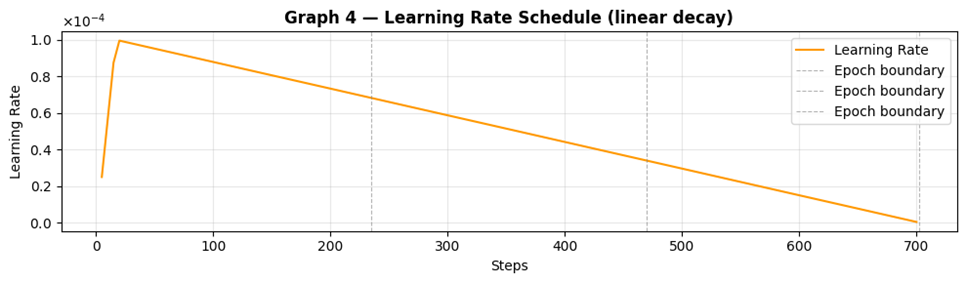
\includegraphics[width=0.8\linewidth]{images/lr_schedule.png}
\caption{Learning rate decay profile (linear warmup + decay)}
\label{fig:lr}
\end{figure}

\subsection{Agentic System Performance}
End‑to‑end evaluation compared our heterogeneous pipeline with a homogeneous baseline (GPT-4o performing both decomposition and section generation).

\begin{table}[htbp]
\centering
\caption{Homogeneous vs. heterogeneous system performance}
\label{tab:comparison}
\begin{tabular}{@{}lcc@{}}
\toprule
Metric & Homogeneous (GPT-4o) & Heterogeneous (Ours) \\
\midrule
Output consistency & Varies with prompt phrasing & Consistent API/naming/styling \\
Inference latency (per section) & 8–16 s & 3–5 s \\
API cost & Non‑trivial per token & Zero (local inference) \\
Orchestration latency & N/A & $<$4 s per decomposition \\
\botrule
\end{tabular}
\end{table}

\textbf{Output consistency:} Qwendean sections showed much higher consistency in component API usage, naming conventions, and Tailwind idioms than GPT-4o sections, which varied with prompt phrasing. A fine‑tuned SLM internalises a consistent coding style from its training corpus, whereas a general‑purpose LLM samples from a broader distribution.

\textbf{Latency and cost:} Section generation on a local RTX 4060 Laptop GPU took 3–5 s per section vs. 8–16 s for GPT-4o API calls—a 3–5× reduction. API cost for Qwendean is effectively zero beyond infrastructure cost.

\textbf{Orchestration quality:} Gemma~4~E2B consistently produced well‑structured section lists with appropriate metadata for e‑commerce, SaaS, and portfolio use cases. The dialogue resolved ambiguities, and decomposition outputs were logical and correctly scoped.

\subsection{Orchestration with Lightweight General‑Purpose Models}
Employing Gemma~4~E2B (2B parameters) for orchestration validates the hypothesis that requirements gathering and structured task decomposition are not compute‑intensive when the problem domain is well‑scoped. The 2B model successfully performed logical reasoning, contextual question formulation, and metadata synthesis. Orchestration latency was under 4 s per decomposition, and handoff to Qwendean was seamless.

This result has far‑reaching implications: functional specialisation, not parameter count, is the source of heterogeneity advantage. A 2B generalist orchestrator + 4B specialist executor outperforms homogeneous architectures of any scale. The efficiency gain comes from matching model capacity to task requirements.

\subsection{Limitations}
\begin{itemize}
    \item Quantitative baselines (pass@k, human preference scores) will be addressed in future work; current evaluation is primarily qualitative.
    \item Dataset size (4100 samples) is sufficient for proof‑of‑concept but not for covering all possible UI components.
    \item Validation currently uses LLM‑based rubric checks; AST/compiler‑level verification is not yet integrated.
\end{itemize}

\section{Future Work}\label{sec:future}

Several directions are identified:
\begin{itemize}
    \item \textbf{Dataset scaling:} Expand to 30,000–40,000 high‑quality samples from additional open‑source libraries, developer‑collected prompts, and adversarial examples.
    \item \textbf{Base model upgrades:} Fine‑tune next‑generation models with better code generation benchmarks.
    \item \textbf{MCP server integration:} Expose Qwendean as a Model Context Protocol (MCP) server, allowing any MCP‑compatible LLM client (Claude, GPT-4o, Gemini) to invoke it as a tool for UI section generation.
    \item \textbf{Code verification layers:} Integrate AST parsing, TypeScript type checking (\texttt{tsc}), and LLM‑based reflection nodes for targeted regeneration.
    \item \textbf{Preference optimisation:} Apply Direct Preference Optimisation (DPO) using human annotations on code readability, reusability, and accessibility.
    \item \textbf{Domain generalisation:} Validate the heterogeneous architecture for API integration code, database schema design, and automated test case generation.
    \item \textbf{Electron demonstration app:} A full desktop application built with Electron has been developed to showcase the end‑to‑end functionality of the heterogeneous agentic pipeline, allowing users to interactively generate UI pages and export React code.
\end{itemize}

\section{Conclusion}\label{sec:conclusion}

We have demonstrated that heterogeneous agentic AI architectures—combining general‑purpose model orchestration with domain‑specific fine‑tuned generation—offer clear advantages over homogeneous architectures for constrained generation problems. For automated UI code generation, our system uses Gemma~4~E2B as a lightweight requirements elicitation and task planner and Qwendean (fine‑tuned Qwen3-4B) as a domain‑specific generator. Qwendean produces consistent, idiomatic, and prompt‑compliant code with much lower inference variance than general‑purpose models.

Crucially, an effective heterogeneous architecture does not require scale‑based heterogeneity. A 2B orchestrator paired with a 4B executor, specialised in its domain, outperforms homogeneous architectures of any scale for well‑defined problems. Orchestrators rely on logical reasoning within a bounded space, which general‑purpose SLMs can handle; code generation requires deep knowledge of syntax, libraries, and idioms, which can be acquired via fine‑tuning.

The development process from 900 to 4,100 multi‑library samples across three training iterations provides practical insights into how dataset quality and diversity affect fine‑tuning dynamics for code generation. The validated configuration (rsLoRA, rank 32, 16‑bit, 3 epochs, 4096 context) is justified by the observed trajectories and quality evaluations. The LangGraph‑based pipeline with Qwendean is a practical, extensible architecture for other domain‑specific heterogeneous AI systems. As LLMs evolve toward tool‑assisted, multi‑agent systems, fine‑tuned SLMs will become increasingly essential for production‑level agentic AI.

\backmatter

\section*{Declarations}

\subsection*{Funding}
Not applicable.

\subsection*{Conflict of interest}
The authors declare no competing interests.

\subsection*{Ethics approval and consent to participate}
Not applicable.

\subsection*{Consent for publication}
All authors consent to publication.

\subsection*{Data availability}
The dataset \texttt{iamdyeus/ui-instruct-4k} and the fine‑tuned model \texttt{iamdyeus/qwendean-4b-GGUF} are publicly available on Hugging Face. Code is available at \url{https://github.com/iamDyeus/qwendean}.

\subsection*{Materials availability}
All materials are open source.

\subsection*{Code availability}
The fine‑tuning and inference code is available at the GitHub repository above.

\subsection*{Author contribution}
\textbf{Arsh:} conceptualisation, methodology, fine‑tuning experiments, training pipeline implementation, LangGraph orchestration, integration of the agentic system, development of the Electron demonstration application, manuscript writing and revision. 
\textbf{Swarnendu Ghosh:} dataset construction, synthetic prompt augmentation (expansion from 900 to 4100 samples), initial LangGraph design, validation support. 
\textbf{Akshay Rajput:} supervision, mentorship, project guidance, and reviewing the manuscript.

\begin{thebibliography}{99}
\bibitem{ref1} P. Belcak and R. Wattenhofer, ``Small Language Models are the Future of Agentic AI,'' \textit{arXiv preprint arXiv:2506.02153}, Jun. 2025.
\bibitem{ref2} J. Wei, X. Wang, D. Schuurmans, et al., ``Chain-of-Thought Prompting Elicits Reasoning in Large Language Models,'' in \textit{Proc. NeurIPS}, Lake Tahoe, NV, USA, Dec. 2022, pp. 1–21.
\bibitem{ref3} LangChain, ``LangGraph: Multi-Agent Orchestration,'' [Online]. Available: https://python.langchain.com/docs/langgraph/. Accessed: Nov. 2025.
\bibitem{ref4} T. Pöppel, M. Eisenschlos, J. Nijkamp, et al., ``On the Transfer Learning Capabilities of Code Models,'' \textit{arXiv preprint arXiv:2409.15895}, Sep. 2024.
\bibitem{ref5} Qwen Team, ``Qwen3 Technical Report,'' \textit{arXiv preprint arXiv:2505.09388}, May 2025.
\bibitem{ref6} DeepSeek-AI, ``DeepSeek-V3 Technical Report,'' \textit{arXiv preprint arXiv:2412.19437}, Dec. 2024.
\bibitem{ref7} R. Rafailov, S. Sharma, H. Zhang, et al., ``Direct Preference Optimization: Your Language Model is Secretly a Reward Model,'' \textit{arXiv preprint arXiv:2305.18290}, May 2023.
\bibitem{ref8} S. Wang, Y. Jiang, H. Xu, Z. Liu, C. C. Elkan, and S. Jain, ``Want To Reduce Labeling Cost for Your Dataset: Read This,'' in \textit{Proc. NeurIPS Datasets and Benchmarks Track}, 2021, pp. 1–15.
\bibitem{ref9} D. D. Ruiz, D. D. García, and J. J. Gómez, ``Automating Web UI Design: Current Approaches and Future Challenges,'' \textit{IEEE Trans. Softw. Eng.}, vol. 49, no. 6, pp. 3150–3170, Jun. 2023.
\bibitem{ref10} ShadCN UI Documentation. [Online]. Available: https://ui.shadcn.com/docs. Accessed: Nov. 2025.
\bibitem{ref11} TailwindCSS Documentation. [Online]. Available: https://tailwindcss.com. Accessed: Nov. 2025.
\bibitem{ref12} E. J. Hu, Y. Shen, P. Wallis, et al., ``LoRA: Low-Rank Adaptation of Large Language Models,'' \textit{arXiv preprint arXiv:2106.09685}, Jun. 2021.
\bibitem{ref13} T. Dettmers, A. Pagnoni, A. Holtzman, and L. Zettlemoyer, ``QLoRA: Efficient Finetuning of Quantized LLMs,'' \textit{arXiv preprint arXiv:2305.14314}, May 2023.
\bibitem{ref14} Unsloth, ``Unsloth: Optimized LLM Fine-Tuning,'' [Online]. Available: https://github.com/unslothai/unsloth. Accessed: Nov. 2025.
\bibitem{ref15} Hugging Face, ``Transformers Library,'' [Online]. Available: https://huggingface.co/docs/transformers. Accessed: Nov. 2025.
\bibitem{ref16} PyTorch Foundation, ``PyTorch Documentation,'' [Online]. Available: https://pytorch.org. Accessed: 2025.
\bibitem{ref17} D. Kalajdzievski, ``A Rank Stabilization Scaling Factor for Fine-Tuning with LoRA,'' \textit{arXiv preprint arXiv:2312.03732}, Nov. 2023.
\end{thebibliography}

\end{document}